\chapter{Validation de la commande en temps continue sur le modèle non linéaire}
\label{ValidationCommande}
%% Chemin d'accès au répertoire : Conception-de-commande\Implémentation Commande Moteur\AGarder\Commandes_matlab
Maintenant que les étapes de démonstration et d'émulation de la commande sont terminés, nous allons étudier notre premier prototype, que nous nommerons prototype 0, et qui correspondra  notre solution 0. Nous allons d'abord effectuer ce que nous appelons un \emph{Model in the loop} où nous allons chercher à améliorer ce premier prototype en utilisant uniquement des simulations. Par la suite, nous améliorerons le prototype en utilisation une technique d'émulation dite \emph{Software in the loop}.
\section{Protocoles MIL/SIL}\label{sec:prtocoleMIL_SIL}
Dans cette partie, nous allons expliquer les démarches que nous utiliserons pour valider nos prototypes. 
	\subsection{Model in the loop (MIL)}
	Pour faire une validation MIL, nous allons utiliser le modèle non linéaire pour simuler la correction. Toute cette opération sera effectué sous MATLAB à l'aide d'un bloc \emph{SIMULINK} qui simule le modèle non linéaire. Pour valider le prototype de commande du correcteur, celui-ci devra respecter la ou les condition que nous lui imposerons. S'il ce n'est pas le cas, une amélioration de ce prototype sera nécessaire et elle nous permettra de créer un prototype N (pour N itérations de cette boucle). 
	Nous devons d'abord fixer une marge d'erreur par rapport au cahier des charges défini en \ref{chap:commande} : 
	\begin{align}\label{eqn_margeErreur}
		M_\epsilon < 1\%
	\end{align}
	Tant que notre prototype ne sera pas en dessous de cette marge, nous devrons le modifier et refaire le test.
	\subsection{SIL}
\section{Test des prototypes des commande à temps continue}
	%	Test des commandes TC sur MNL et Moteur
	% 	Utilisation protocoles MIL  (ne le ré-explique pas)  
	%			The PLAN
	A présent, nous pouvons commencer à tester les prototypes de commandes du moteur sur des modèles plus complexe : nous disposons pour cela d'un modèle non linéaire ainsi que d'un banc moteur. Nous suivront les consignes que nous venons de présenter en \ref{sec:prtocoleMIL_SIL}, en commençant par présenter le moyen utilisé pour adapter la simulation. 
	Comme il est évoqué dans le titre de cette section, nous sommes ici en temps continu. Les hypothèses pour la discrétisation ne sont pas traités dans cette partie, nous avons choisi de construire le prototype de commande à temps discret quand nous aurons d'abord validé complètement la commande en temps continu, et que nous auront présenté toutes les contraintes que la discrétisation devra surmonter. %% TODO - ref vers parti discrétisation.
	\subsection{Simulation sur Modèle Non linéaire}
		
		Nous disposons de la démarche que nous allons utiliser pour valider notre simulation. Pour cette partie, nous utiliserons un bloc \emph{SIMULINK} qui nous permettra de simuler un modèle très proche du banc moteur. Ce modèle n'a pas reçu les simplifications que posent les hypothèses faites en \ref{sub:linearisation} et en \ref{sub:invariance}. Un bloc \emph{SIMULINK} est disponible à cet effet, sous forme de \emph{S-Function}. Il utilise la modélisation et les paramètres utilisés en \ref{sub:equationPhysique} pour créer un système Entrées/Sorties beaucoup plus proche que le modèle linéaire d'ordre 4. 
		% Image et mesure
		\subsubsection{Adaptation modèle}
		% Encapsulation de la commande ?
		Pour permettre l'utilisation de ce modèle, nous devons d'abord lancer une compilation de la \emph{S-function}. Cette opération est nécessaire car la \emph{S-function} est un code en langage C qui s'adapte à la simulation \emph{SIMULINK}, et êrmet ainsi d'obtenir des performances en temps de calcul plus élevé qu'en bloc de simulation classique.
		Nous avons choisi d'en-capsuler tout le bloc de commande (Gain du retour d'état et reconstruction d'état) dans un bloc \emph{sub-system} que nous détaillons en annexe \ref{annex:modl_NL_SIMULINK}. Ce sous bloc prend en entrée 2 signaux : la consigne de référence $y_ref$ et la sortie mesuré du système $y_m = V_s$ (Position du moteur, cf chapitre \ref{chap:modelisation}), et calcule la commande qu'il émet sur le connecteur nommé $u$.\begin{figure}[ht]
		\centering
		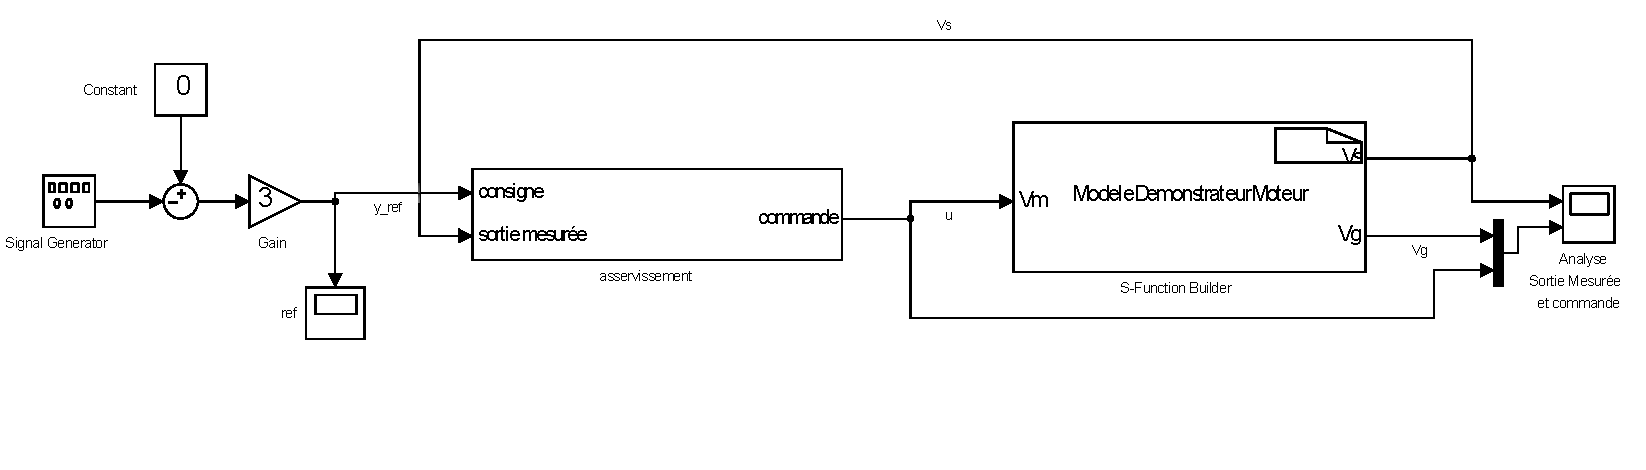
\includegraphics[width = \textwidth]{./IV/images/NL_RE_BlocEntier.pdf}
		\caption{Schéma \emph{SIMULINK} complet de l'asservissement du modèle du moteur Non linéaire}\label{fig:SIMULINK_NL_schema}
		\end{figure}
		
		Nous avons placé des points de mesure au sur le signal de référence ainsi qu'en sortie du système. Nous obtenons ainsi une réponse temporelle que nous allons étudier dans la sous section suivante.
		\subsubsection{Simulation et étude de performances}
		Utilisons maintenant la simulation précédente pour étudier les performances de notre commande. Nous avons dans un premier temps observer la reconstruction d'état du système et nous avons pu noter un problème. %TODO 
		
		% Changement des valeurs propres.
			
		% Nouvelle simulation.
		Une nouvelle simulation faite sur ce nouveau prototype nous donne les résultats montré dans la figure \ref{fig:SimuNL_ref_sortieVS_VM}. Nous pouvons voir une erreur sur le régime permanent qui subsiste toujours. Ce léger décalage devrait pouvoir être corrigé sur un modèle linéaire avec un ajout d'un gain pur compenser ce manque. Or, nous sommes sur un modèle non linéaire et cette méthode ne peut pas fonctionner. 
		\begin{center}
		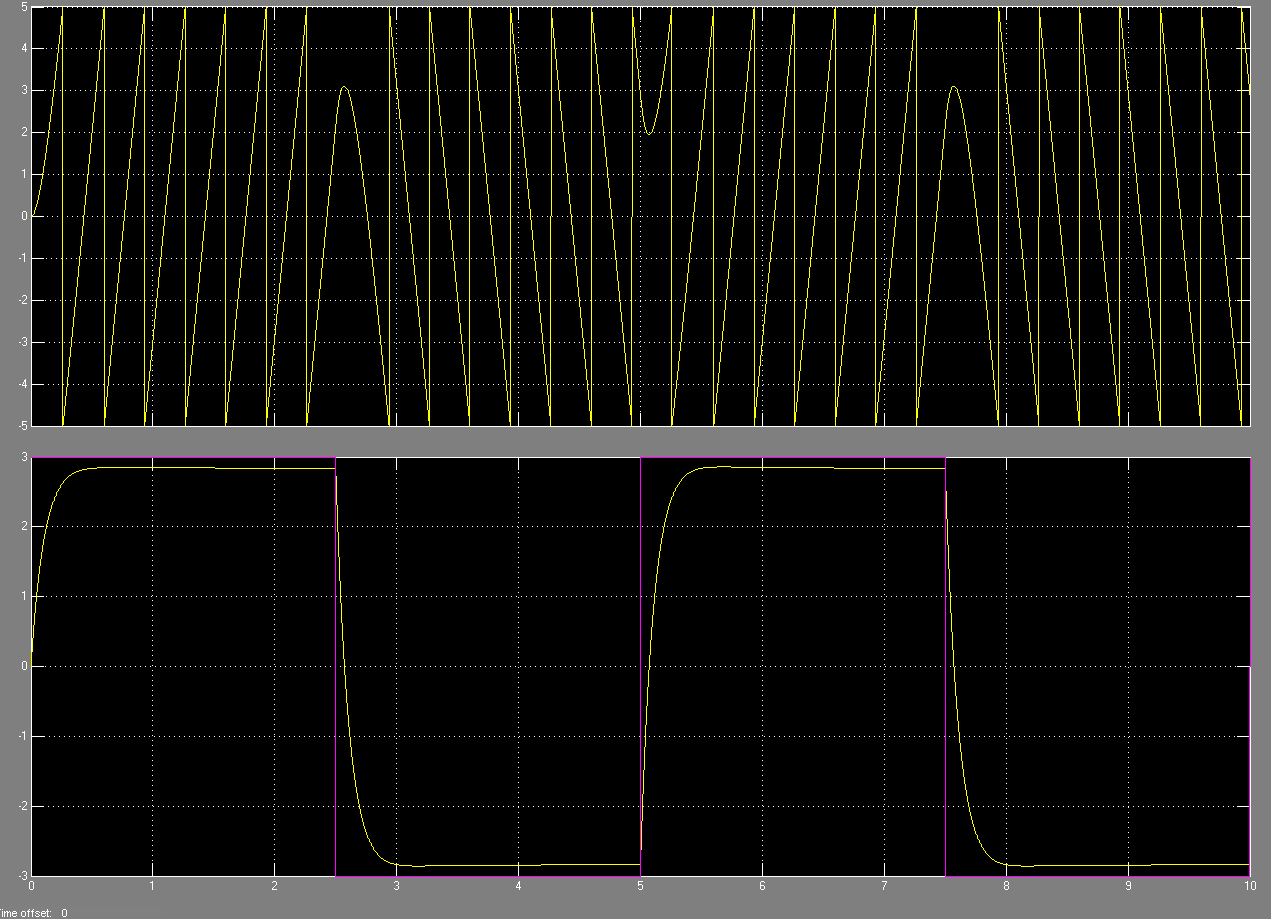
\includegraphics[width= .8\textwidth]{./IV/images/NL_Position--ref_sortie_RE.PNG}
		\captionof{figure}{Simulation des signaux $V_s$ (Bloc du haut), de $y_{ref}$(Bloc du bas/courbe violet) et de $V_m$(Bloc du bas/courbe jaune)\label{fig:SimuNL_ref_sortieVS_VM} }
		\end{center}		
		
		Un zoom sur l'erreur du régime permanent, disponoble en annexe \ref{annex:modl_NL_SIMULINK} - figures \ref{fig:SIMULINK_NL_erreur_reponse} et \ref{fig:SIMULINK_NL_erreur_reponse_zoom}, nous indique que pour une consigne $y_{ref} = 3$, nous obtenons $V_m(t_f)\approx 2.85$. Nous avons donc une erreur en régime statique \begin{align*}
		\epsilon = \frac{y_{ref}}{V_m(t_f)} = 5\%
		\end{align*}
		\subsubsection{Conclusion et Validation}
	\subsection{Simulation sur moteur Réel}
		Nous souhaitons maintenant améliorer notre prototype avec le banc moteur directement. En utilisant la fonction de prototypage rapide de MATLAB, nous sommes capables de générer une émulation du micro contrôleur. Celui ci va s'occuper de récupérer les sorties mesurées du banc moteur, calculer la commande correspondantes et la générer sur l'entrée de commande du moteur. 
		\subsubsection{Adaptation du modèle}
		\subsubsection{Test et étude de performances}
		\subsubsection{Conclusion et Validation}
		
%\chapter{Planification de la suite de l'asservissement}
%\label{chap:suite}
%Dans ce chapitre, nous allons décrire les étapes suivantes à cette étude théorique. Dans un premier temps sera présenté la validation de notre commande par tests puis il sera abordé les étapes nécessaires à l'implémentation sur micro-contrôleur et la validation finale.
%\section{Validation de commande}
%Dans un premier temps, nous testerons notre asservissement sur un modèle plus riche (non linéaire, variant, plus de dynamique, ...) en simulation afin de voir si notre commande respecte toujours le cahier des charges. Le modèle sera fournie en seconde séance de TP. Ensuite, nous testerons le moteur dans différentes configurations en fonction des résultats et de notre vitesse d'avancement : 
%\begin{itemize}
%\item Émulation sur le même ordinateur (test du temps concret).
%\item Test de la commande et du procédé sur un même ordinateur en sortant le signal de commande par les cartes d'entrées/sorties du prototypage rapide.
%\item Test de la commande simulée sur un ordinateur et le procédé simulé sur un second ordinateur afin de tester deux vitesses de fonctionnement de simulation (synchronisations) et les cartes entrées/sorties (communications).
%\item Test de la commande simulée et le procédé simulé sur un micro-contrôleur.
%\item Test de la commande simulée sur procédé réel : on éprouve ici la robustesse de la commande face aux imprécisions de modélisation.
%\end{itemize}
%Nous effectuerons aussi une estimation du modèle de comportement du moteur que nous asservirons afin d'avoir un modèle plus proche du comportement réel.
%\section{Implémentation sur micro-contrôleur}
%% CAN CNA
%% Fech et F micro c
%% MODELE Z 
%% PROG
%% ORDO
%% IMPLE
%
%Dans cette partie, nous appréhenderons les problématiques de conversions de signaux numériques/analogiques et analogiques/numériques et essaierons de les corriger afin d'avoir des conversions les plus linéaires possibles. Nous calculerons les fréquences maximales et minimales des entrées et sorties du procédé, cela nous permettra de choisir des fréquences de conversions adaptées et la fréquence de fonctionnement du micro-contrôleur. Nous transformerons aussi notre modèle de commande en un modèle à temps discret afin de pouvoir l'implémenter. Une fois le modèle temps discret obtenu, nous programmerons les différentes fonctions nécessaires à l'asservissement (lecture des entrées, calcul des sorties, écriture des sorties). Nous aborderons aussi les problématiques d'ordonnancement afin que notre programme puisse s'exécuter dans le temps impartie afin de respecter les contraintes temps réels. Enfin, nous implémenterons notre programme sur le micro-contrôleur C167.
%\section{Validation finale}
%Une fois la commande implémentée, nous effectuerons les tests suivants : 
%\begin{itemize}
%\item Test de la commande implémentée sur le procédé simulé sur ordinateur.
%\item Test de la commande implémentée sur le procédé simulé sur micro-contrôleur.
%\item Test de la commande implémentée sur la maquette du procédé réel.
%\end{itemize}
%
%Nous vérifierons le respect des spécifications du cahier des charges dans l'ensemble de ces tests afin de voir si notre asservissement est correct.